%%% Time-stamp: <2015-04-15 00:55:14 sunthar>

%%% $Log:$

%\documentclass[11pt,a4paper,openright]{report}
\documentclass[seminar,twoside]{iitbreport}


%% Selectively comment out sections that you want to be left out but
%% maintaining the page numbers and other \ref
\includeonly{%
  chapter1/introduction,
  chapter2/background,
  chapter3/techniques,
  chapter4/management,
  chapter5/conclusion
}  
%expt/experimental,
%rnd/results,


%%% Some commonly used packages (make sure your LaTeX installation
%%% contains these packages, if not ask your senior to help installing
%%% the packages)


\usepackage{booktabs}
\usepackage{url}
\graphicspath{{expt/}}


%%% Macro definitions for Commonly used symbols
\newcommand{\etas}{\ensuremath{\eta_{\mathrm{s}}}}
\newcommand{\Rey}{\ensuremath{\mathrm{Re}}}
\newcommand{\avg}[1]{\ensuremath{\overline{#1}}}
\newcommand{\tenpow}[1]{\ensuremath{\times 10^{#1}}}

\newcommand{\pder}[2]{\ensuremath{\frac{\partial#1}{\partial#2}}}


% Referencing macros
\newcommand{\Eqref}[1]{Equation~\eqref{#1}}
\newcommand{\Tabref}[1]{Table~\ref{#1}}
\newcommand{\Figref}[1]{Figure~\ref{#1}}
\newcommand{\Appref}[1]{Appendix~\ref{#1}}

\def\myurl{\hfil\penalty100 \hfilneg\hbox}

%Command for including image source
\newcommand{\captionsource}[3]{%
  \caption[{#1}]{%
	#2%
    \\\hspace{\linewidth}%
   	%\textbf{Source:}\hspace{2pt}%
    \myurl{#3}%
	%#3	
	}%
}

\begin{document}
\title{Study of Virtualization \& Management of Memory in Virtualized Systems}
\author{Aby Sam Ross\\143050093}
%\date{\today}
\degree{Master of Technology}
\dept{Computer Science \& Engineering}
\monthyear{April 2015}

%\makecoverpage
\maketitle

\begin{abstract}
Memory like other computing resources can be considered a scarce enough commodity. Multiplexing
and management of this memory among various stakeholders in native computing environments has been
well taken care of. But when it comes to virtualized environments it adds another layer of
abstraction. This calls for new techniques, for partitioning and arbitrating memory among
different VMs, that doesn't change the OS's perspective of the scheme of things and requires
minimal changes. While the techniques for partitioning memory among different VMs in a virtualized
setting has almost got standardized, there are still differing views and different approaches to
managing memory. The new layer of abstraction introduced by virtualization adds considerable
complexity in estimating the needs and utilization of memory. One cannot retrofit one strategy
suitable for a particular setting to another and expect to get a clear picture of memory related
parameters. This seminar is to understand different techniques of memory virtualization and to gain some insight into some of the existing management strategies.
 
\end{abstract}

\pagenumbering{roman}
\tableofcontents

%\listoftables
\listoffigures

%\cleardoublepage
\clearpage
\setcounter{page}{1}
\pagenumbering{arabic}


\chapter{Introduction}

\section{Overview of Virtualization}
Hardware resource abstraction and management have always been a major aim and challenge in
electronic systems. With the advent of computers these tasks fell upon a huge piece of software
called the Operating System. It became the responsibility of the OS to multiplex the resources
among the different processes running in a system. An obvious illustration is that of CPU
multiplexing, where the CPU is scheduled in time slices among various processes according to
priority. The physical memory in a system as well is a resource. Memory also needs to be
abstracted and suitable interfaces are to be provided for easy and efficient use. Traditionally
this has been achieved through the concept of virtual memory coupled with paging or segmentation.
\\
With advancements in technology the capabilities of physical resources increased and cost
decreased. Processors and memory became faster, smaller chips with more capacity became available.
But these advancements didn't percolate naturally into better utilization of these resources.
Often these resources were underutilized. In order to get better utility from these resources
various options of sharing these resources at a larger granularity was explored. Thus came into
existence the concept of virtualization.\\
Virtualization increases the granularity of abstraction from individual resources to abstracting
the entire set of hardware as a single unit or in other words virtualization abstracts the entire
computer system. With this we could have more than one machine running on top of the existing
computing hardware. These machines came to be called \textit{Virtual Machines} or VM. In other
words with the increase in granularity of abstraction the unit of allocation to the abstraction
increased from a process to an entire OS.\\
The ringmaster who runs the show in a Virtual Machine is still the humongous piece of code called
the OS. But traditionally OSes were designed to have ownership and control of the underlying
hardware. Virtualization now created a separation between the hardware and the OS.They were now
relegated to the status of a \textit{guest OS}. A single OS was no longer the sole owner and
controller of the resources. The entire hardware had to be abstracted, interfaced and multiplexed
among different OSes manning different VMs analogous to the way in which an OS enabled
multiplexing of resources among different processes in a native system. This role was now taken up
by a new, but no less hideous, software layer called the \textit{Virtual Machine Monitor} (VMM) or
the \textit{Hypervisor}. That is now we have the hypervisor sitting on top of the hardware 
directly and above it we have different VMs.\\
The introduction of a new orchestrator, the Hypervisor, and relegation of a guest OS to a lesser
privilege brought about new challenges. The guest OS in a VM had no longer complete control of the
underlying resources to arbitrate efficiently among the processes running in it. But to the
process local to a VM the guest OS was still the ringmaster who ran the show. Hence it became of
paramount importance that the introduction of a software layer, the hypervisor, between the guest
OS and the resources didn't break the equivalence view  i.e. a process running in a VM should see
no or little difference in running on a native vs. virtualized system. At the same time we also
had to ensure that every VM stayed within its allocated bounds and guest OS operations had enough
efficiency. These requirements of hypervisor design are formally stated in 
\cite{popek1974formal}.The hypervisor can choose from among the various strategies like
instruction interpretation, trap \& emulate, binary translation, para-virtualization, hardware
assisted virtualization to provide the aforementioned requirements.\\
Once such a hypervisor is available efficient resource utilization and management comes next in
order to meet the original design principles of virtualization. Memory like other
resources will also be apportioned to the different VMs. But it is not necessary that all  of the
memory allocated to a VM will be in 100\% use all the time. This gives us an opportunity to
reallocate this unused memory to other VMs in need. But its sharing and management is not as
simple as that of a flexible resource like CPU and nor are the effects of differences in the
amounts of memory available that easily visible \citep{hwang2013mortar}. The objective of this
seminar is to get an understanding of the intricacies involved in this. 

\section{Scope of the Seminar}
The objective of this seminar is not to delve deep into the implementation of virtualization as a
whole but rather to concentrate on understanding how memory virtualization is achieved, the pros and cons of different techniques of memory virtualization, optimizations to it, challenges of memory management in virtualized systems, memory reallocation mechanisms, and some of the existing memory management strategies.     

%\begin{itemize}
%\item Unnumbered and Numbered Lists
%\item Equations
%\item Defining short macros for frequently used symbols
%\item Bibliography
%\item Figures
%\item Tables
%\end{itemize}

%The normal procedure for compiling a \LaTeX\ document that contains
%bibliographic entries is to follow the following steps
%\begin{enumerate}
%\item \verb|pdflatex mainrep|
%\item \verb|bibtex mainrep|
%\item \verb|pdflatex mainrep|
%\item \verb|pdflatex mainrep|
%\end{enumerate}
%In the above example \verb|mainrep| is the main \LaTeX\ file.




%This is the first chapter, which resides in a directory (folder)
%intro. Each chapter can contain \verb|section|, \verb|subsection|
%and so on.




%Equations should be set in a separate mode.  For details on getting
%various types of aligned equations, consult the \AmS-\LaTeX\
%documentation \verb|amsldoc.pdf|. Simple equations are set as
%\begin{equation}
%\label{eq:sinx}
%\int \mathrm{d}x \; \cos x =  \sin x
%\end{equation}
%Equation~\eqref{eq:sinx} is the integral of the cosine
%function. Mathematical symbols must always be put inside \verb|$$|,
%when they appear outside a math environment (such as \verb|equation|,
%\verb|align|, \verb|gather|, etc).  The symbol ``ex'' must be written as
%$x$ and not as x.  

%Another commonly used construct for equations is the \verb|align|
%environment to align several equations along a vertical line. It is
%usually the $=$ sign across which the alignment is done.  The
%point of alignment for each equation is specified using the ampersand symbol 
%\begin{align}
%a &= b  \\
%a + e + f + g & = m + n + z \\
%x + 2 & = x^{3} + 3 x^{2} + 2 x + 5
%\end{align}

%\subsection{Commonly used Symbols}
%For mathematical symbols it is very convenient to define frequently
%used symbols as a short macro. For example if you are to be using the
%symbol $\eta_{\mathrm{s}}$ frequently it is convenient to define it in
%as:\\
%\verb|\newcommand{\etas}{\ensuremath{\eta_{\mathrm{s}}}}| \\
%n the preamble and to simply refer it to in the text as \etas\ or in
%a mathematical equation as $\etas = \eta \, ( 1 + \phi)$.

%%% Local Variables: 
%%% mode: latex
%%% TeX-master: "../mainrep"
%%% End: 

\chapter{Background}

\section{Memory Management in Native Systems}
Memory management in non-virtualized native multiprogramming system is achieved using Virtual
Memory. In multiprogrammed systems several programs are resident in memory at the same time.
The memory management policy in such a system deals with protecting the memory of one program from 
another, loading a program into available space in main memory, de/allocating memory dynamically
from/to programs.\\
While programs are complied and linked with addresses starting at $0$ and CPU uses 
these addresses to access the binary, it isn't necessary (and is the not the case that) that a
program will get physical memory with the same addresses or it is not even guaranteed that there
will be enough space in the physical memory to load the entire binary of the program. Most of the
times only the immediately needed part of the program is loaded onto the available physical
memory, (the rest will be held in a backing store - often the hard disk) and they will share the
physical memory space along with parts of other programs. And the OS may choose to evict parts of
the program to the backing store when in need of memory as a part of its memory management policy.
Therefore the addresses generated by CPU needs to be translated into the corresponding physical
addresses. The address generated by CPU is called \textit{Virtual Address} or VA . Thus we need to
have a mechanism of \textit{Virtual Address (VA)} $\rightarrow$ \textit{Physical Address (PA)}
translation.\\
Hence the illusion that is given to a program that there is enough physical memory available to
store its entire binary combined with relocation of code having contiguous virtual addresses into
- not necessarily contiguous - available physical memory chunks are the central ideas of virtual
memory.\\
Virtual Memory can be implemented in more than one ways. Paging is one of them. The idea behind
paging is to divide the virtual address space and the physical memory into same sized units of
allocation called \textit{pages}. Hence the virtual address space is divided into \textit{virtual
pages} or simply \textit{pages} and physical memory into \textit{physical pages} or
\textit{frames} or \textit{physical/machine frames}. It is thus clear that not all pages of a
program will be present in the physical memory when the program is executing, the contiguous
virtual pages belonging to the same program needn't be allocated contiguous frames and it is
necessary to provide a way to map from the virtual pages to the associated machine frames.\\
This mapping should be there for each program and this mapping is called the \textit{page table}.
The organisation of page table is closely tied to the size of a page or a frame. Page size is
taken as \textit{power of 2} as this ensures that all binary representable addresses can be
utilized and address manipulation can be done without arithmetic operations. There should an be an
entry for all virtual page addresses of a program in its page table. This will result in a very
long (large) page table and all the page tables of all programs that are currently resident in
memory will consume considerable amount of physical memory. So instead of storing such a single
large page table per program in memory we break the page tables into different levels to have a
tree like structure. Thus following the design principles of virtual memory it is not necessary
that even all the levels of the page table will be resident in memory all the time.\\
Often the entries in each level are grouped into different sets. And each entry will contain a
physical address and some flag bits. The flag bits store permissions and other info about the this
entry and the physical address in the entry points to a set of entries in the next level. These
sets of entries in each level are often limited to single physical frame. Thus the physical
address in a page table entry points to a physical frame in the next level. There is an exception
for the last level of the page table. An entry in the last level contains the physical address of
the actual virtual page that we were looking for and the flag bits of the entry include
information like whether the physical page it points to is present or not. The physical address of
the root of the page table (i.e. the physical address of the base of the outermost level of page
table) is stored in a hardware register.\\
The translation of virtual address to physical address happens in the following manner:\\
The base address of the program's page table is obtained from the hardware register storing it. To
this base address we add that part of the virtual address that corresponds to the outermost level. 
Thus we get the corresponding entry in the outer most level which points to the base address of
the corresponding set of entries of the next level (i.e. a physical page of the next level) . Now
to get to the corresponding entry within that physical page we add the part of virtual address for
the next level to the physical page address we obtained from the outermost level. This process is
continued till we get to a last level entry from which we get the physical frame address 
corresponding to the virtual address. And to go to the exact physical address location
corresponding to the virtual address location add the last part of the virtual that doesn't
correspond to any page table level i.e. the offset part to the physical frame address.\\    
Hence it is clear from the above discussion that the parts of the virtual address that correspond
to each level of page table give us an offset within that level and last part of the virtual
address that doesn't correspond to any page table level gives us the offset within the actual
frame that holds this virtual address. Illustration in figure ~\ref{fig:fig1}.\\
For a virtual address generated by the CPU the translation to physical address i.e. traversing the
levels of page table happens in hardware. If the corresponding physical page is present in the
translated location it is a \textit{hit} else it is a \textit{fault}. Page faults are to be
resolved by moving in the corresponding missing page from the backing store. Certain architectures
like x86 choose to cache recently accessed virtual addresses and their mappings in a small cache
often called the \textit{translational look ahead buffer} or TLB, this is for faster translations
the next the same address is accessed. This also brings about the need for coherence between the
entries in the TLB and the page table. The hardware that does all this is called the
\textit{memory management unit} or MMU.\\
Linux OS on x86 (i.e. 32 bit) architecture has 3 levels of the page table. While for x86\_64 (i.e.
64bit) it has 4. They are called \textit{page global directory} or PGD, \textit{page upper
directory} or PUD, \textit{page middle directory} or PMD and \textit{page table entry} or PTE. x86
won't have the PMD. The \textit{CR3} register holds the base address of the PGD.\\
\begin{figure}[tbp]
  \begin{center}
    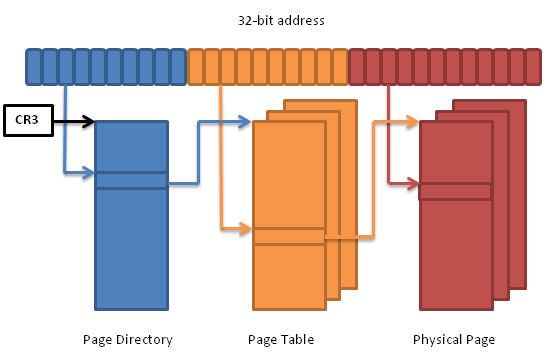
\includegraphics[width=0.7\textwidth]{pagetable}
    \caption[Page Table Illustration]{Illustration of \textit{VA} $\rightarrow$ \textit{PA} address translation.}
    \label{fig:fig1}
  \end{center}
\end{figure}


\chapter{Memory Virtualization}

\section{Physical Memory Allocation Model in Virtualized Systems} \label{model}
Since within a VM the guest OS provides its application the virtual memory abstraction and
processes running in the guest OS share what the guest OS perceives as the physical memory, the
guest OS is allowed to maintain the mapping of virtual addresses to what it perceives as its
physical memory. But as explained earlier the guest OS is tricked into believing that it is
managing a real contiguous physical memory just as the way in normal virtual memory scenario a
process is tricked by the OS into believing that it is loaded on and executing from physically
contiguous machine memory.\\
Hence the guest OS's perception of physical memory is actually a pseudo-contiguous-physical memory
abstraction provided by the VMM. As per common virtualization terminology it is called
\textit{guest physical frames} and a corresponding page number is called \textit{Guest Physical
Frame Number} or GPFN. And the corresponding original machine frame number backing a GPFN is
termed machine frame number or MFN. Thus the guest OS page page tables contains the \textit{virtual address} $\rightarrow$ \textit{guest physical address} mapping also abbreviated as V $\rightarrow$ P mapping and the VMM should contain a \textit{guest physical address} $\rightarrow$ \textit{machine address} mapping often abbreviated as P $\rightarrow$ M. The P $\rightarrow$ M mapping should be maintained from the time a VM is created and should be updated every time a change occurs to the allocation of machine frames to a VM. This is illustrated in figure \ref{fig:allocmodel}.

\begin{figure}[tbp]
  \begin{center}
    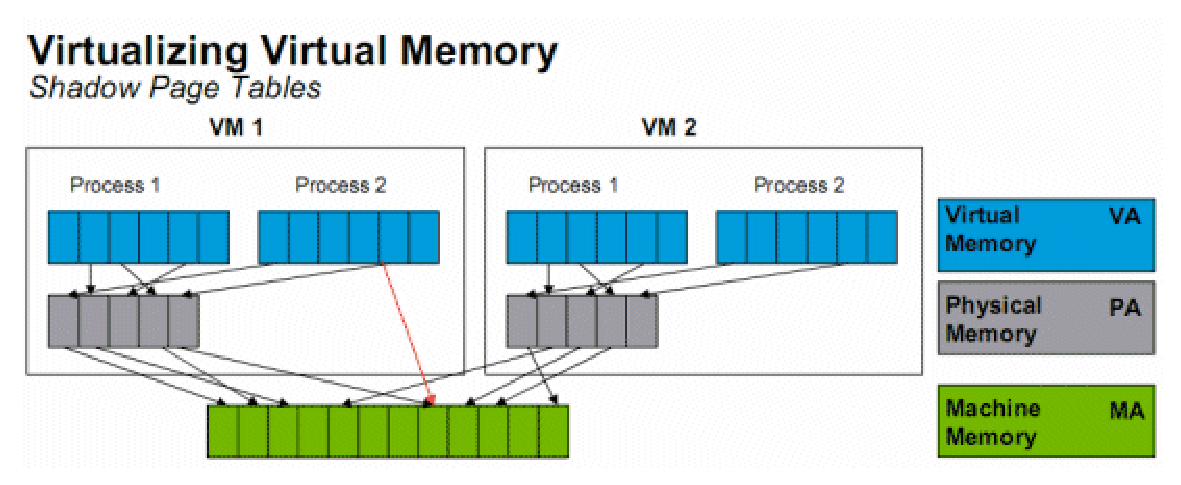
\includegraphics[width=0.7\textwidth]{images/allocmodel}
        	%\caption[Page Table Illustration]{Illustration of \textit{VA} $\rightarrow$ \textit{PA} address translation.}
    		\captionsource{Virtualized Physical Memory Allocation Model}{Physical memory allocation model in virtualized systems.}%
    		{\url{images.anandtech.com/reviews/it/2008/virtualization-nuts-bolts/Shadowpt.gif}}  
    \label{fig:allocmodel}
     \end{center}
\end{figure}

\section{Techniques of Virtualizing the MMU} \label{techniques}
This section discusses how the hypervisor defines ways for the guest OS to access the actual
machine frames through the MMU functionalities provided by it.\\
We know that the guest OS maintains page table related information for every process running in a
VM and also that the guest OS operates on pseudo physical pages or GPFNs. Memory references by
processes running in a VM  requires translation of virtual addresses into machine addresses via
hardware MMU operations such as page table walk. The page table walk itself needs actual machine
frames addresses to get to the different levels of page table as discussed in \ref{native}. But as
discussed in \ref{challenges} the guest OS cannot be given unrestricted direct access to the
machine frames holding the page table pages to ensure VM isolation. This means that the guest OS
access to the actual MMU (or its functionalities) in the VMM, like CR3 access, changes to page
table entries need to be supervised by the VMM.\\
Table \ref{tab:tech} lists the existing methodologies of virtualizing MMU.
\begin{table}[tbp]
  \begin{center}
    \caption{MMU virtualization techniques.}
    \label{tab:tech}
    \begin{tabular}{ll}
      \toprule 
      Technique & Description \\
      \midrule
      Shadow Paging & Software approach\\
      Direct Paging &  Para-virtualization approach\\
      Nested Page Tables & Hardware assisted approach\\
      \bottomrule \\
    \end{tabular}
  \end{center}
\end{table}
\subsection{Shadow Paging} \label{sp}
Shadow paging mechanism is a software MMU virtualization mechanism.
The access to CR3 is by default protected by design paradigms of virtualization which pushed the
guest OS to lower privilege levels than the hypervisor. The machine frames that contain the
different page table levels are protected by making them write protected. And for each
process in a VM, just like a guest OS maintains a page table, the hypervisor also maintains a page
table called the \textit{Shadow Page Table}. The shadow page table is part of a plan to easily get
the direct the V $\rightarrow$ M mapping instead of going through \textit{V} $\rightarrow$
\textit{P} and then \textit{P} $\rightarrow$ \textit{M} as mentioned in \ref{model}. Ideally every
virtual address that is translated to corresponding guest physical page address in the guest OS
should be translated to the corresponding machine frame address via P $\rightarrow$ M in the VMM.
This applies to guest physical page addresses that correspond to the pages of the guest OS page
table as well. But there is a subtle drawback to this approach. To translate a virtual address we
know that the guest OS needs to access the page table whose base address is stored in the CR3.
Assuming we have access to the CR3, for the time being, can we go ahead and directly access the
guest page table? No, because what the guest OS have is only the guest physical page address of
the the page table base. What we need is the address of the machine frame that holds this guest
physical page. And in order to access it we need to do a translation using the P $\rightarrow$ M
mappings. This needs to be repeated for the base address of every level of the page table.\\
In order to alleviate this overhead we make use of the same P $\rightarrow$ M mappings maintained
by the VMM for a VM to create shadow page tables for all process that run in that VM. And in
the shadow page tables we maintain the direct V $\rightarrow$ M mappings. Thus every virtual
address access by a process in a VM can now go through the corresponding shadow page table in the
VMM saving on the number of memory accesses and the corresponding latency. Figure
\ref{fig:shadowpagetables} illustrates this.\\
\begin{figure}[tbp]
  \begin{center}
    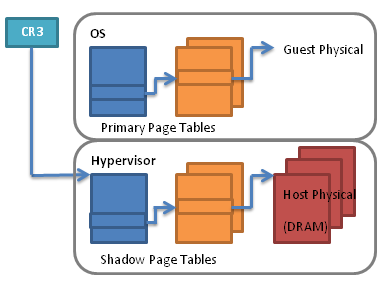
\includegraphics[width=0.7\textwidth]{images/shadowpagetables}
        	%\caption[Page Table Illustration]{Illustration of \textit{VA} $\rightarrow$ \textit{PA} address translation.}
        	\captionsource{Shadow Page Table Illustration}{Shadow Page Table Illustration.}{\url{corensic.files.wordpress.com/2011/12/shadowpagetables.png}}  
    \label{fig:shadowpagetables}
     \end{center}
\end{figure}
To pull off this trick the guest OS's CR3 is virtualized and guest OS access to the CR3 is to be
prevented by a general protection fault (GPF) \citep{wiki1}. The VMM should load the CR3 with the
base address of the shadow page table rather than with the base of guest OS page table. Virtual
memory access that reads or writes already mapped frames can go ahead via the shadow page table
unhindered. When a page fault occurs the VMM checks if the guest page table has valid entries for
the faluting address, if that is the case then fault occurred because the VMM had moved the
machine frame corresponding to the faulting address to its swap space. This type of fault should
be hidden from the guest OS as such a fault would not have occurred if the guest OS was running on
a native system. The VMM now swaps in the contents of the faulting address into machine memory,
updates the P $\rightarrow$ M mapping to reflect this and the updates the corresponding shadow
page table. On the other hand if the fault occurred because the guest page table did not have
valid mappings for this virtual address, the VMM transfers control to the trap handler of the
guest indicating a page fault. The guest OS will then issues I/O requests to effect a page-in
operation, which may or may not cause a dirty page swap out. These requests are in fact serviced
by the VMM as they are privileged instructions. Once the guest physical page (and the machine
frame backing it is) is available the guest OS issues instructions to the modify the guest page
tables \citep{smith2005virtual}. This causes an exception called \textbf{VMExit} as the frames
containing guest page tables are write protected from the guest OS. The VMM now updates the guest
page table and the mappings in the shadow page table before returning control back to the guest.
This is done to ensure that the shadow page table is in sync with the guest page table.  
\subsection{Direct Paging} \label{para}
Direct Paging uses an approach called \textit{Para-Virtualization} in which the guest OS
is made aware of being virtualized. Guest OS is modified as a part of the MMU virtualization. This
approach makes use of the \textbf{VMCALL} or \textit{hypercall} API provided by para-
virtualization. This is a solution to the x86 architecture virtualization issue. More
can be read from \citet{force2000analysis}.\\
The major change that this brings about is in the way in which guest page tables are updated.
There is no shadow page table in this approach. Here also the machine frames containing the guest
page tables are write protected by making them read only. A change to the guest page table are
carried out by a VMCALL from the guets OS to the VMM. Subsequently the VMM VMCALL handler carries
out the changes to the corresponding machine frames after validating them to ensure isolation.
Hence the guest page tables contains direct \textit{virtual address} $\rightarrow$ \textit{machine
address} mappings that are VMM validated. As it is the case with shadow paging mechanism
normal page table reads happen without VMM intervention and page faults are handled by the guest
OS by updating the page table entries through the VMM. Figure \ref{fig:para} illustrates this
approach.
\begin{figure}[tbp]
  \begin{center}
    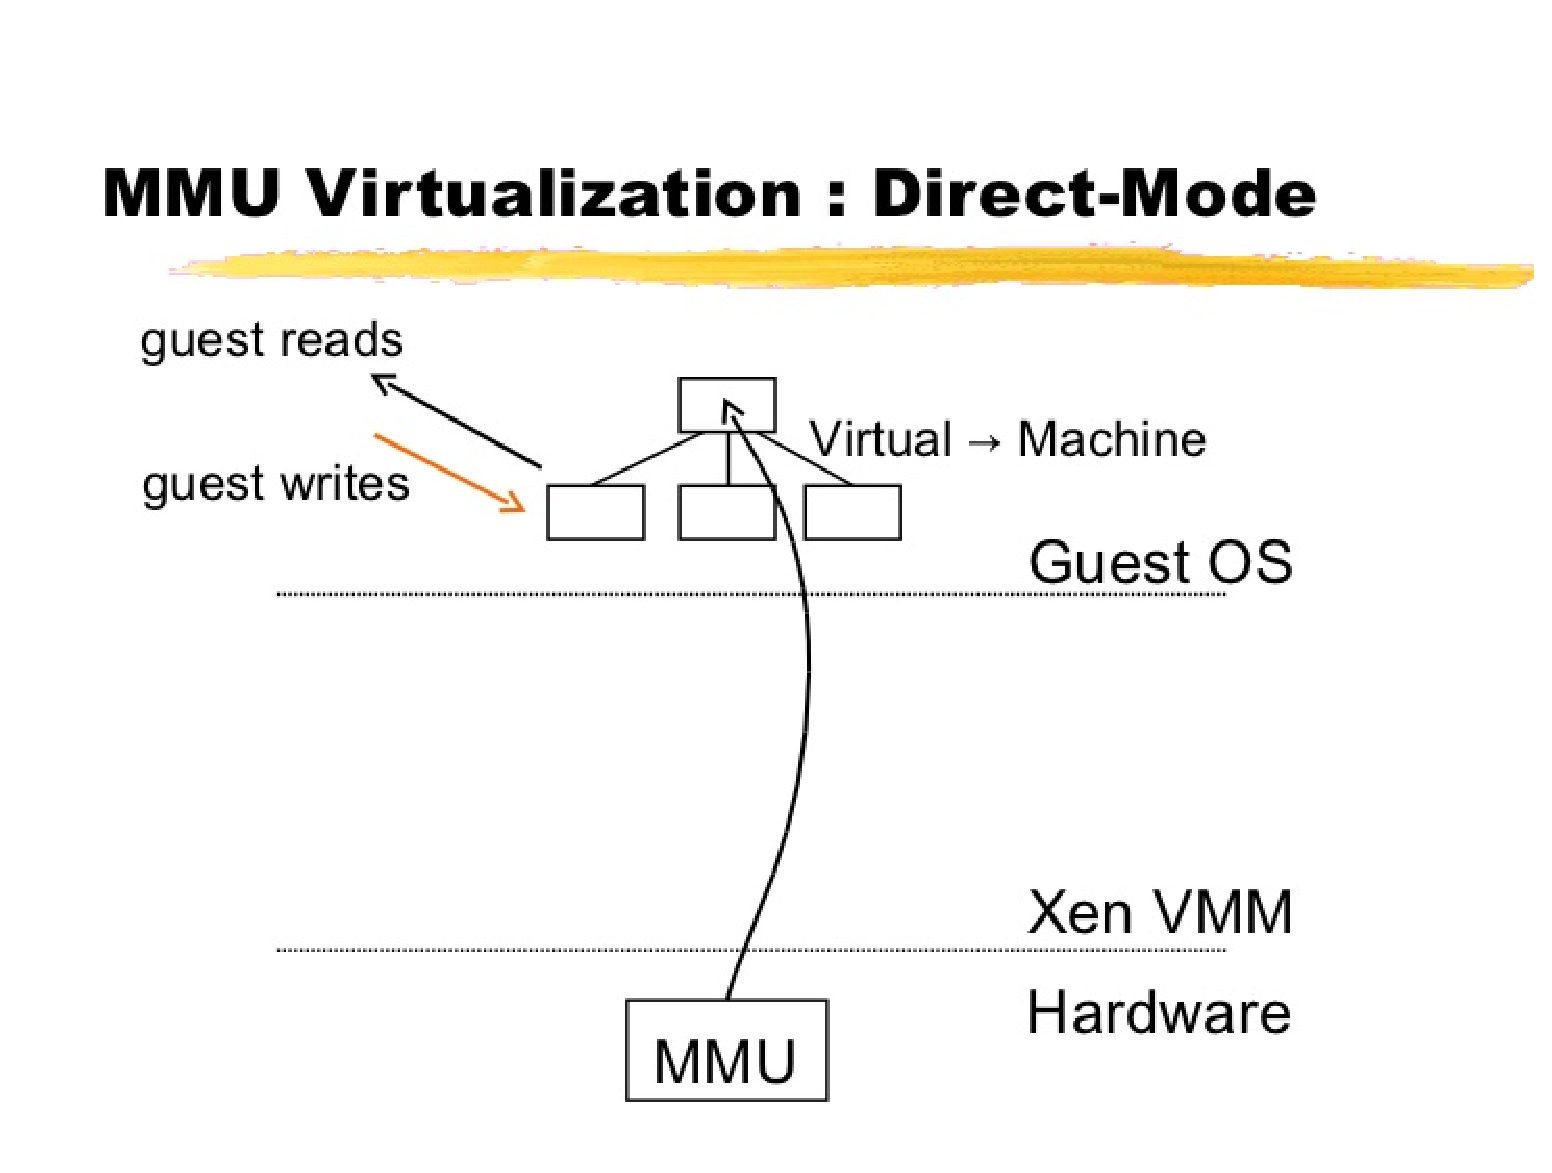
\includegraphics[width=0.7\textwidth]{images/paravirt}
        	%\caption[Page Table Illustration]{Illustration of \textit{VA} $\rightarrow$ \textit{PA} address translation.}
        	\captionsource{Direct Mapping Illustration}{Direct Mapping Illustration.}{\url{image.slidesharecdn.com/overview-of-xen-30627/95/overview-of-xen-30-12-728.jpg}}  
    \label{fig:para}
     \end{center}
\end{figure}
\subsection{Nested Page Tables} \label{nested}
Extensions to the hardware in the form \textit{extended page tables or nested page tables} (EPT or
NPT) enabled a new mechanism to achieve memory virtualization called \textit{hardware assisted MMU
virtualization}. Contrary to shadow paging, nested paging removes the need for the VMM to
supervise the guest OS page table operations once the nested pages are populated. Under nested
paging both guest and the hypervisor have their own copy of the CR3 register. The guest OS maps
virtual addresses to guest physical addresses and the Nested page tables (NPT) map guest physical
addresses to machine frame addresses. The guest now is allowed to set up the guest page tables
without any hindrance (i.e VMExits) by the VMM, except for getting a physical frame allocated (for
the guest page table or any other guest physical page) which is still under the preview of the
VMM. The VMM sets up the nested page table. A guest OS virtual memory reference, when nested page
tables are set up, results in a 2-D page table walk - first in the guest page table and next in
the nested page table - to get to the corresponding machine frame. Parts of virtual address is
used to index into the guest page tables, as explain in \ref{native}, to obtain the guest physical
address and using this guest physical address we do a similar indexing into the nested page table
to obtain the machine frame address. There is a subtle issue here that may miss our eyes easily.
While translating a virtual address we need to access machine frames holding the guest page table
pages, so for each level of guest page table accessed we need to do a nested page table walk to
reach the machine frame holding this page table page.\\
If the guest page tables contain \textit{n levels} and the nested page table contains \textit{m
levels}, then to resolve a virtual address to corresponding machine frame we require \[((n+1)\ *\
m) + n\] memory accesses. For getting the machine frame address of a particular level of guest
page table physical page we need to traverse \textbf{n} levels of nested page table. Once the
machine frame is identified we need 1 memory access for reading it. These are the \textbf{n + 1}
memory accesses in the previous expression. This is repeated for all levels of guest page table.
Hence the \textbf{(n+1) * m}. Once you reach the machine frame which holds the last level of guest
page table i.e. the PTE machine frame you can read the guest physical address of the original
virtual address address and finally to obtain its machine address we need to traverse the nested
page tables one last time. That is why the \textbf{n} term is added to the equation.
This is illustrated in figure \ref{fig:npt}.\\
\begin{figure}[tbp]
  \begin{center}
    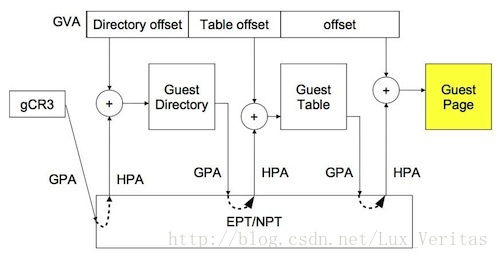
\includegraphics[width=0.7\textwidth]{images/npt}
        	%\caption[Page Table Illustration]{Illustration of \textit{VA} $\rightarrow$ \textit{PA} address translation.}
        	\captionsource{Nested Page Table Illustration}{Nested Page Table Illustration.}{\url{cnblogs.com/snake-hand/p/3181631.html}}  
    \label{fig:npt}
     \end{center}
\end{figure}

\section{Comparison of Memory Virtualization Techniques}
Following table compares the different memory virtualization techniques.
\begin{table}[!htbp]
  \begin{center}
    \caption{Comparing Memory Virtualization Techniques.}
    \label{tab:compare}
    \begin{tabular}{p{3cm} p{5cm} p{5cm}}
      \toprule 
      Technique & Advantage & Disadvantage \\
      \midrule
      Shadow Paging & Software approach, no changes to guest OS  & Frequent costly VMExits for each guest page table updation.\\
      \midrule
      Direct Paging &  No VMExits & Requires changes to the guest OS.\\
      \midrule
      Nested Page Tables & Hardware assisted approach, No VMExits, No changes to guest OS. & More number of memory for a virtual memory translation. About 6 times more. \\
      \bottomrule \\
    \end{tabular}
  \end{center}
\end{table}
\section{Optimizations to Memory Virtualization Techniques}
Shadow Paging and Nested Page Tables are two approaches that doesn't require changes to the guest
OS. The solution approach they take, though seems similar, are independent of each other. If a 
process running in the guest OS is experiencing large number of page faults then shadow paging is
going to degrade the performance because of frequent VMExits required to synchronize the guest and
shadow page tables (refer \ref{sp}). Hence shadow paging will prove to be a bad memory
virtualization technique for such a process. Now consider another scenario where a process is
experiencing large number of TLB misses but its pages are still in memory i.e. it has few page
faults, then resolving their machine address by doing a 2-D page table walk in nested paging
mechanism is going to degrade its performance due to increased number of memory accesses (refer
\ref{nested}). For this process nested paging proves to be a bad choice of memory virtualization
technique.
\subsection{Combining Shadow Paging \& Nested Page Table}
Neither of the two strategies is a clear winner all the time for different mix of processes
possible in a VM. Hence in order to get the best of these two techniques \citet{wang2011selective}
proposes a dynamic switching mechanism that switches between the shadow paging and nested paging
based on memory access behaviour of the VMs and they call it the \textit{Dynamic Switching Paging}
or DSP. Their solution approach is as follows:
\begin{itemize}
\item Determine page fault frequency and TLB miss frequency measured as the number of page faults
and the number of TLB misses per thousand retired (finished) instructions.
\item Determine system dependent upper and lower thresholds for page faults frequency \& TLB miss
frequency.
\item If one metric is beyond its upper threshold \& the other is well within within its threshold
limits, then switch to the technique/mode that is the most suitable for the metric that is within
its limits.
\begin{itemize}
\item ``If the TLB miss frequency is higher than the TLB miss upper-bound threshold and the page
fault frequency is lower than 80 percent of the page fault upper-bound threshold, switch from''
nested page table mode to shadow page table mode or stay in shadow page table mode if already in
it.
\item ``If the page fault frequency is higher than the page fault upper-bound threshold and the
TLB miss frequency is lower than 80 percent of the TLB miss upper-bound threshold, switch from''
shadow paging mode to nested page table mode or stay in nested page table mode if already in it.  
\end{itemize}
\item If both metrics are below their lower threshold limits then remain in the current mode. 
\item If both metrics are above their upper threshold values or within their threshold limits find
out the relative penalty between them.
\item Calculate the relative penalty as the P-to-T ratio. \[P-to-T ratio\ =\ \frac{Page\ Fault\ 
Frequency}{TLB\ Miss\ Frequency}\]
\item P-to-T ratio is used along with a running average of recent P-to-T ratios called historic P-
o-T ratios.
\item If either of historic TLB miss frequency or current TLB miss frequency is zero then switch
from shadow paging to nested page tables without estimating either historic or current P-to-T
ratio. This avoids divide by zero errors.
\item If both historic and latest P-to-T ratio are above P-to-T ratio threshold upper bound switch
from shadow paging to nested page tables or stay in nested page tables if already in it.
\item If both historic and latest P-to-T ratio are lower than P-to-T ratio threshold lower bound
switch from nested page tables to shadow paging or stay in shadow paging mode if already in it.
\item If both historic and latest P-to-T ratio are within the P-to-T ratio threshold's lower \&
upper bounds stay in current mode.
\item If historic and latest P-to-T ratio falls into different threshold intervals, a clear trend
cannot be estimated and hence it is better to stay back in current mode.     
\end{itemize}
Through experimentations they claim that DSP is capable of matching the performance of the better
among shadow paging and nested page tables, though they do not explain clearly how they attributed
the performance degradation of particular processes to the memory virtualization technique used.
\subsection{Reducing the number of Memory Accesses while using Nested Page Table}     
+
\include{chapter4/management}
\include{chapter5/conclusion}
%\chapter{Results and Discussion}


\section{Including Tables}

Tables are to be used in a special environment so that they have a
Number, caption and appear in the list of tables.
Table~\ref{tab:samtab} is a sample table. In the case of tables, it is
a convention to write the caption above the table.  Note that in the
case of figures the caption appears below the figure.

\begin{table}[tbp]
  \begin{center}
    \caption{Physical properties of the materials used.}
    \label{tab:samtab}
    \begin{tabular}{ll}
      \toprule 
      Property & Value \\
      \midrule
      Particle Density, $\rho_{\mathrm{p}}$ & 2500 kg/m$^{3}$ \\
      Viscosity, $\eta_{\mathrm{s}}$& 1 $\times 10^{-3}$ Pa-s \\
      \bottomrule \\
    \end{tabular}
  \end{center}
\end{table}

%%% Local Variables: 
%%% mode: latex
%%% TeX-master: "../mainrep"
%%% End: 


\bibliography{mainrep}


\end{document}




%%% Local Variables: 
%%% mode: latex
%%% TeX-master: t
%%% End: 
